\documentclass{tufte-handout}

\title{CS224n: Natural Language Processing with Deep Learning\thanks{Course Instructors: Christopher Manning, Richard Socher}}

\author[Rohit Mundra, Richard Socher]{Lecture Notes: Part III\thanks{Author: Rohit Mundra, Amani Peddada, Richard Socher,  Qiaojing Yan}}

\date{Winter 2017} % without \date command, current date is supplied

%\geometry{showframe} % display margins for debugging page layout

\usepackage{graphicx} % allow embedded images
  \setkeys{Gin}{width=\linewidth,totalheight=\textheight,keepaspectratio}
  \graphicspath{{notes3/fig/}} % set of paths to search for images
\usepackage{amsmath}  % extended mathematics
\usepackage{amstext}  % extended text
\usepackage{booktabs} % book-quality tables
\usepackage{units}    % non-stacked fractions and better unit spacing
\usepackage{multicol} % multiple column layout facilities
\usepackage{lipsum}   % filler text
\usepackage{fancyvrb} % extended verbatim environments
\usepackage{placeins}
\usepackage{mdframed}% http://ctan.org/pkg/mdframed
  \fvset{fontsize=\normalsize}% default font size for fancy-verbatim environments

% Standardize command font styles and environments
\newcommand{\doccmd}[1]{\texttt{\textbackslash#1}}% command name -- adds backslash automatically
\newcommand{\docopt}[1]{\ensuremath{\langle}\textrm{\textit{#1}}\ensuremath{\rangle}}% optional command argument
\newcommand{\docarg}[1]{\textrm{\textit{#1}}}% (required) command argument
\newcommand{\docenv}[1]{\textsf{#1}}% environment name
\newcommand{\docpkg}[1]{\texttt{#1}}% package name
\newcommand{\doccls}[1]{\texttt{#1}}% document class name
\newcommand{\docclsopt}[1]{\texttt{#1}}% document class option name
\newenvironment{docspec}{\begin{quote}\noindent}{\end{quote}}% command specification environment
\newcommand{\argmin}{\operatornamewithlimits{argmin}}
\newcommand{\argmax}{\operatornamewithlimits{argmax}}
\newcommand{\norm}[1]{\left\lVert#1\right\rVert}
\newcommand{\textunderscript}[1]{$_{\text{#1}}$}
\allowdisplaybreaks
\setcounter{secnumdepth}{3}

\newmdtheoremenv[outerlinewidth=2,leftmargin=40,rightmargin=40,%
    backgroundcolor=lightgray,outerlinecolor=blue,innertopmargin=10pt,%
    splittopskip=\topskip,skipbelow=\baselineskip,%
    skipabove=\baselineskip,ntheorem,roundcorner=5pt]{theorem}{Snippet}[section]

\begin{document}

\maketitle% this prints the handout title, author, and date

%\printclassoptions


\textbf{Keyphrases: Neural networks. Forward computation. Backward propagation. Neuron Units. Max-margin Loss. Gradient checks. Xavier parameter initialization. Learning rates. Adagrad.}\\

\noindent{}This set of notes introduces single and multilayer neural networks, and how they can be used for classification purposes. We then discuss how they can be trained using a distributed gradient descent technique known as backpropagation. We will see how the chain rule can be used to make parameter updates sequentially. After a rigorous mathematical discussion of neural networks, we will discuss some practical tips and tricks in training neural networks involving: neuron units (non-linearities), gradient checks, Xavier parameter initialization, learning rates, Adagrad, etc. Lastly, we will motivate the use of recurrent neural networks as a language model.

\section{Neural Networks: Foundations}\label{sec:nnets}

\begin{marginfigure}%
  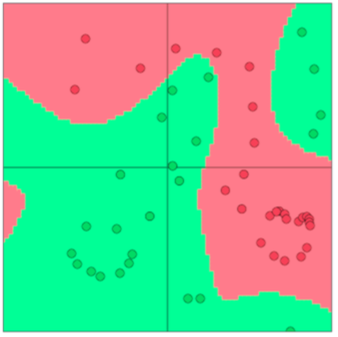
\includegraphics[width=\linewidth]{NonlinearBoundary}
  \caption{We see here how a non-linear decision boundary separates the data very well. This is the prowess of neural networks.}
  \label{fig:NonlinearBoundary}
\end{marginfigure}

\marginnote{\textbf{Fun Fact:}\\ Neural networks are biologically inspired classifiers which is why they are often called "artificial neural networks" to distinguish them from the organic kind. However, in reality human neural networks are so much more capable and complex from artificial neural networks that it is usually better to not draw too many parallels between the two.}

We established in our previous discussions the need for non-linear classifiers since most data are not linearly separable and thus, our classification performance on them is limited. Neural networks are a family of classifiers with non-linear decision boundary as seen in Figure~\ref{fig:NonlinearBoundary}. Now that we know the sort of decision boundaries neural networks create, let us see how they manage doing so.

\subsection{A Neuron}\label{sec:neuron}

A neuron is a generic computational unit that takes $n$ inputs and produces a single output. What differentiates the outputs of different neurons is their parameters (also referred to as their weights). One of the most popular choices for neurons is the "sigmoid" or "binary logistic regression" unit. This unit takes an $n$-dimensional input vector $x$ and produces the scalar activation (output) $a$. This neuron is also associated with an $n$-dimensional weight vector, $w$, and a bias scalar, $b$. The output of this neuron is then:
$$ a = \frac{1}{1 + \exp(-(w^Tx + b))}$$
\marginnote{\textbf{Neuron:}\\A neuron is the fundamental building block of neural networks. We will see that a neuron can be one of many functions that allows for non-linearities to accrue in the network.}
We can also combine the weights and bias term above to equivalently formulate:
$$ a = \frac{1}{1 + \exp(-[w^T~~~b] \cdot[x~~~1])}$$

\begin{marginfigure}%
  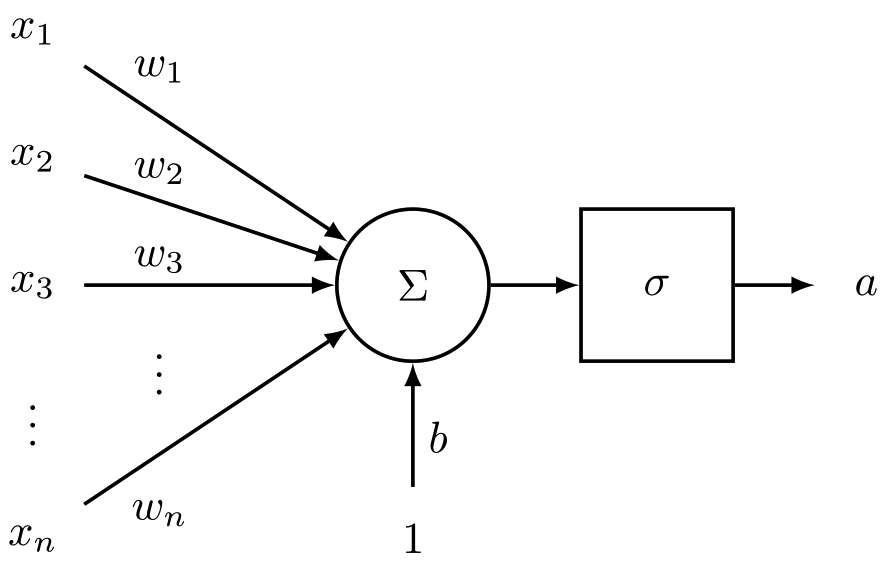
\includegraphics[width=\linewidth]{sigmoidneuron}
  \caption{This image captures how in a sigmoid neuron, the input vector $x$ is first scaled, summed, added to a bias unit, and then passed to the squashing sigmoid function.}
  \label{fig:sigmoidneuron}
\end{marginfigure}

This formulation can be visualized in the manner shown in Figure~\ref{fig:sigmoidneuron}.

\subsection{A Single Layer of Neurons}\label{sec:neuronlayer}

We extend the idea above to multiple neurons by considering the case where the input $x$ is fed as an input to multiple such neurons as shown in Figure~\ref{fig:SingleLayerNeuralNetwork}. 

If we refer to the different neurons' weights as $\{w^{(1)}, \cdots, w^{(m)}\}$ and the biases as $\{b_1, \cdots, b_m\}$, we can say the respective activations are  $\{a_1, \cdots, a_m\}$:
\begin{align*}
a_1 &= \frac{1}{1 + \exp(w^{(1)T}x + b_1)}\\
\vdots \\
a_m &= \frac{1}{1 + \exp(w^{(m)T}x + b_m)}
\end{align*}
Let us define the following abstractions to keep the notation simple and useful for more complex networks:
\begin{align*}
\sigma(z) &= \begin{bmatrix}  \frac{1}{1 + \exp(z_1)}\\ \vdots \\  \frac{1}{1 + \exp(z_m)}\end{bmatrix}\\
b &= \begin{bmatrix}  b_1\\ \vdots \\  b_m \end{bmatrix} \in \mathbb{R}^{m}\\
W &= \begin{bmatrix} - & w^{(1)T} & -\\ & \cdots & \\ - & w^{(m)T} & - \end{bmatrix} \in \mathbb{R}^{m\times n}
\end{align*}
We can now write the output of scaling and biases as:
\begin{marginfigure}%
  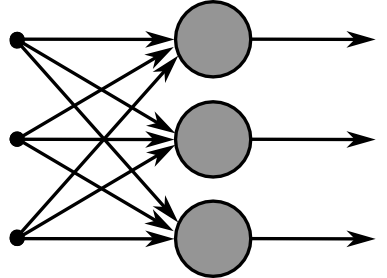
\includegraphics[width=\linewidth]{SingleLayerNeuralNetwork}
  \caption{This image captures how multiple sigmoid units are stacked on the right, all of which receive the same input $x$.}
  \label{fig:SingleLayerNeuralNetwork}
\end{marginfigure}
$$z = Wx + b$$
The activations of the sigmoid function can then be written as:
$$\begin{bmatrix}  a^{(1)}\\ \vdots \\  a^{(m)} \end{bmatrix} = \sigma (z) = \sigma (Wx + b)$$

So what do these activations really tell us? Well, one can think of these activations as indicators of the presence of some weighted combination of features. We can then use a combination of these activations to perform classification tasks.

\subsection{Feed-forward Computation}\label{sec:ff}

So far we have seen how an input vector $x \in \mathbb{R}^n$ can be fed to a layer of sigmoid units to create activations $a \in \mathbb{R}^m$. But what is the intuition behind doing so? Let us consider the following named-entity recognition (NER) problem in NLP as an example:

\begin{center}
\textit{"Museums in Paris are amazing"}
\end{center}

\marginnote{\textbf{Dimensions for a single hidden layer neural network:}
If we represent each word using a $4$-dimensional word vector and we use a $5$-word window as input, then the input $x \in \mathbb{R}^{20}$. If we use $8$ sigmoid units in the hidden layer and generate $1$ score output from the activations, then $W \in \mathbb{R}^{8\times 20}$, $b \in \mathbb{R}^{8}$, $U \in \mathbb{R}^{8\times 1}$, $s \in \mathbb{R}$.  The stage-wise feed-forward computation is then:\\
$$z = Wx + b$$
$$a = \sigma(z)$$
$$s = U^Ta$$
}

Here, we want to classify whether or not the center word \textit{"Paris"} is a named-entity. In such cases, it is very likely that we would not just want to capture the presence of words in the window of word vectors but some other interactions between the words in order to make the classification. For instance, maybe it should matter that \textit{"Museums"} is the first word only if \textit{"in"} is the second word. Such non-linear decisions can often not be captured by inputs fed directly to a Softmax function but instead require the scoring of the intermediate layer discussed in Section~\ref{sec:neuronlayer}. We can thus use another matrix $U \in R^{m\times 1}$ to generate an unnormalized score for a classification task from the activations:
$$s = U^Ta = U^T f(Wx + b)$$
where $f$ is the activation function. 

\begin{marginfigure}%
  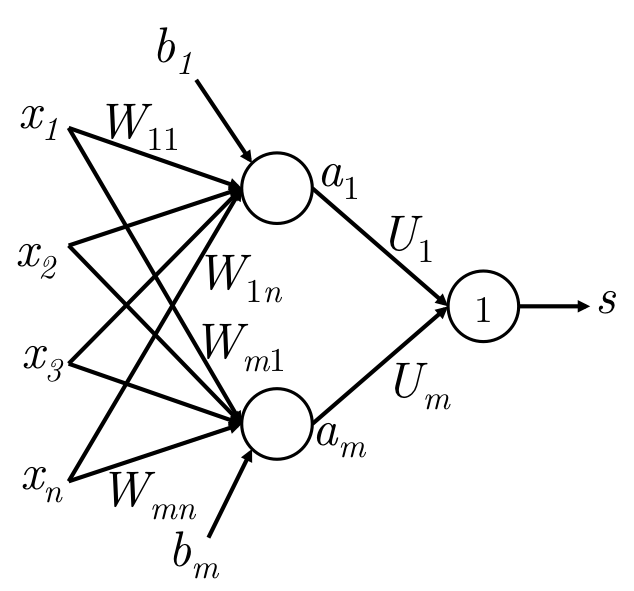
\includegraphics[width=\linewidth]{SimpleFF}
  \caption{This image captures how a simple feed-forward network might compute its output.}
  \label{fig:SimpleFF}
\end{marginfigure}

\textbf{Analysis of Dimensions: }If we represent each word using a $4$-dimensional word vector and we use a $5$-word window as input (as in the above example), then the input $x \in \mathbb{R}^{20}$. If we use $8$ sigmoid units in the hidden layer and generate $1$ score output from the activations, then $W \in \mathbb{R}^{8\times 20}$, $b \in \mathbb{R}^{8}$, $U \in \mathbb{R}^{8\times 1}$, $s \in \mathbb{R}$.

\subsection{Maximum Margin Objective Function}\label{sec:maxmargin}

Like most machine learning models, neural networks also need an optimization objective, a measure of error or goodness which we want to minimize or maximize respectively. Here, we will discuss a popular error metric known as the maximum margin objective. The idea behind using this objective is to ensure that the score computed for "true" labeled data points is higher than the score computed for "false" labeled data points. 

Using the previous example, if we call the score computed for the "true" labeled window \textit{"Museums in Paris are amazing"} as $s$ and the score computed for the "false" labeled window \textit{"Not all museums in Paris"} as $s_c$ (subscripted as $c$ to signify that the window is "corrupt").

Then, our objective function would be to maximize $(s - s_c)$ or to minimize $(s_c - s)$. However, we modify our objective to ensure that error is only computed if $s_c > s \Rightarrow (s_c - s) > 0$. The intuition behind doing this is that we only care the the "true" data point have a higher score than the "false" data point and that the rest does not matter. Thus, we want our error to be $(s_c - s)$ if $s_c > s$ else 0. Thus, our optimization objective is now:
$$\operatornamewithlimits{minimize} J = \max(s_c - s, 0)$$

However, the above optimization objective is risky in the sense that it does not attempt to create a margin of safety. We would want the "true" labeled data point to score higher than the "false" labeled data point by some positive margin $\Delta$. In other words, we would want error to be calculated if $(s - s_c < \Delta)$ and not just when $(s - s_c < 0)$. Thus, we modify the optimization objective:
$$\operatornamewithlimits{minimize} J = \max(\Delta+s_c - s, 0)$$
We can scale this margin such that it is $\Delta = 1$ and let the other parameters in the optimization problem adapt to this without any change in performance. For more information on this, read about functional and geometric margins - a topic often covered in the study of Support Vector Machines.
\marginnote{The max-margin objective function is most commonly associated with Support Vector Machines (SVMs)}
Finally, we define the following optimization objective which we optimize over all training windows:
$$\operatornamewithlimits{minimize} J = \max(1+s_c - s, 0)$$
In the above formulation $s_c = U^T f(Wx_c + b)$ and $s = U^T f(Wx + b)$.


\subsection{Training with Backpropagation -- Elemental}\label{sec:backprop1}
In this section we discuss how we train the different parameters in the model when the cost $J$ discussed in Section~\ref{sec:maxmargin} is positive. No parameter updates are necessary if the cost is $0$. Since we typically update parameters using gradient descent (or a variant such as SGD), we typically need the gradient information for any parameter as required in the update equation:
$$ \theta^{(t+1)} = \theta^{(t)} - \alpha \nabla_{\theta^{(t)}}J$$
Backpropagation is technique that allows us to use the chain rule of differentiation to calculate loss gradients for any parameter used in the feed-forward computation on the model. To understand this further, let us understand the toy network shown in Figure~\ref{fig:421nnet} for which we will perform backpropagation.
\begin{marginfigure}%
  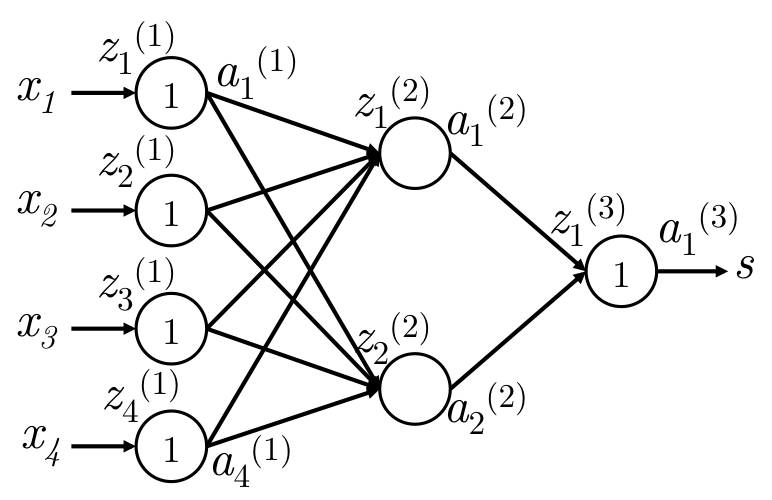
\includegraphics[width=\linewidth]{421nnet}
  \caption{This is a 4-2-1 neural network where neuron $j$ on layer $k$ receives input $z_{j}^{(k)}$ and produces activation output $a_{j}^{(k)}$.}
  \label{fig:421nnet}
\end{marginfigure}

Here, we use a neural network with a single hidden layer and a single unit output. Let us establish some \textbf{notation} that will make it easier to generalize this model later:
\begin{itemize}
\item $x_i$ is an input to the neural network.
\item $s$ is the output of the neural network.
\item Each layer (including the input and output layers) has neurons which receive an input and produce an output. The $j$-th neuron of layer $k$ receives the scalar input $z_j^{(k)}$ and produces the scalar activation output $a_j^{(k)}$.
\item We will call the backpropagated error calculated at $z_j^{(k)}$ as $\delta_j^{(k)}$. 
\item Layer 1 refers to the input layer and not the first hidden layer. For the input layer, $x_j = z_j^{(1)} = a_j^{(1)}$.
\item $W^{(k)}$ is the transfer matrix that maps the output from the $k$-th layer to the input to the  $(k+1)$-th Thus, $W^{(1)} = W$ and $W^{(2)} = U$ to put this new generalized notation in perspective of Section~\ref{sec:ff}.
\end{itemize}

\marginnote{\textbf{Backpropagation Notation:}\\
\begin{itemize}
\item $x_i$ is an input to the neural network.
\item $s$ is the output of the neural network.
\item The $j$-th neuron of layer $k$ receives the scalar input $z_j^{(k)}$ and produces the scalar activation output $a_j^{(k)}$.
\item For the input layer, $x_j = z_j^{(1)} = a_j^{(1)}$.
\item $W^{(k)}$ is the transfer matrix that maps the output from the $k$-th layer to the input to the  $(k+1)$-th. Thus, $W^{(1)} = W$ and $W^{(2)} = U^T$ using notation from Section~\ref{sec:ff}.
\end{itemize}
}

\textbf{Let us begin:} Suppose the cost $J = (1 + s_c - s)$ is positive and we want to perform the update of parameter $W^{(1)}_{14}$ (in Figure~\ref{fig:421nnet} and Figure~\ref{fig:ErrorSignal}), we must realize that $W^{(1)}_{14}$ only contributes to $z_1^{(2)}$ and thus $a_1^{(2)}$. This fact is crucial to understanding backpropagation -- backpropagated gradients are only affected by values they contribute to. $a_1^{(2)}$ is consequently used in the forward computation of score by multiplication with $W^{(2)}_{1}$. We can see from the max-margin loss that:
$$\frac{\partial J}{\partial s} = - \frac{\partial J}{\partial s_c} =  -1$$
Therefore we will work with $\frac{\partial s}{\partial W^{(1)}_{ij}}$ here for simplicity. Thus,
\begin{align*}
\frac{\partial s}{\partial W^{(1)}_{ij}} &= \frac{\partial W^{(2)} a^{(2)}}{\partial W^{(1)}_{ij}} = \frac{\partial W^{(2)}_{i} a^{(2)}_i}{\partial W^{(1)}_{ij}} = W^{(2)}_{i} \frac{\partial a^{(2)}_i}{\partial W^{(1)}_{ij}}\\
\Rightarrow W^{(2)}_{i} \frac{\partial a^{(2)}_i}{\partial W^{(1)}_{ij}} &=  W^{(2)}_{i} \frac{\partial a^{(2)}_i}{\partial z^{(2)}_i} \frac{\partial z^{(2)}_i}{\partial W^{(1)}_{ij}}\\
&=  W^{(2)}_{i} \frac{f(z^{(2)}_i)}{\partial z^{(2)}_i} \frac{\partial z^{(2)}_i}{\partial W^{(1)}_{ij}}\\
&=  W^{(2)}_{i} f'(z^{(2)}_i) \frac{\partial z^{(2)}_i}{\partial W^{(1)}_{ij}}\\
&=  W^{(2)}_{i} f'(z^{(2)}_i) \frac{\partial}{\partial W^{(1)}_{ij}} (b^{(1)}_i + a_1^{(1)}  W^{(1)}_{i1} + a_2^{(1)}  W^{(1)}_{i2} + a_3^{(1)}  W^{(1)}_{i3} + a_4^{(1)}  W^{(1)}_{i4})\\
&=  W^{(2)}_{i} f'(z^{(2)}_i) \frac{\partial}{\partial W^{(1)}_{ij}} (b^{(1)}_i + \sum_k a_k^{(1)}  W^{(1)}_{ik})\\
&=  W^{(2)}_{i} f'(z^{(2)}_i) a_j^{(1)}\\
&=  \delta_i^{(2)} \cdot a_j^{(1)}
\end{align*}
We see above that the gradient reduces to the product $\delta_i^{(2)} \cdot a_j^{(1)}$ where $\delta_i^{(2)}$ is essentially the error propagating backwards from the $i$-th neuron in layer 2. $a_j^{(1)}$ is an input fed to $i$-th neuron in layer $2$ when scaled by $W_{ij}$.

\begin{marginfigure}%
  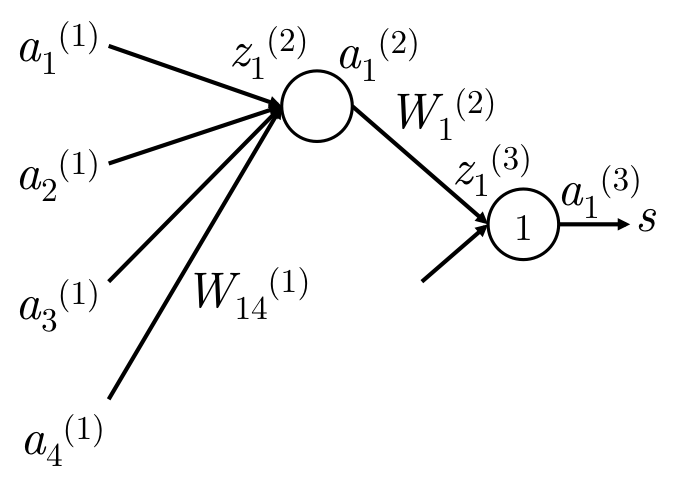
\includegraphics[width=\linewidth]{ErrorSignal}
  \caption{This subnetwork shows the relevant parts of the network required to update $W^{(1)}_{ij}$}
  \label{fig:ErrorSignal}
\end{marginfigure}

Let us discuss the "error sharing/distribution" interpretation of backpropagation better using Figure~\ref{fig:ErrorSignal} as an example. Say we were to update $W^{(1)}_{14}$:
\begin{enumerate}
\item We start with the an error signal of 1 propagating backwards from $a_1^{(3)}$.
\item We then multiply this error by the local gradient of the neuron which maps $z_1^{(3)}$ to $a_1^{(3)}$. This happens to be $1$ in this case and thus, the error is still 1. This is now known as $\delta_1^{(3)} = 1$.
\item At this point, the error signal of 1 has reached $z_1^{(3)}$. We now need to distribute the error signal so that the "fair share" of the error reaches to $a_1^{(2)}$.
\item This amount is the (error signal at $z_1^{(3)} = \delta_1^{(3)}$)$ \times W_{1}^{(2)} = W_{1}^{(2)}$. Thus, the error at $a_1^{(2)} = W_{1}^{(2)}$.
\item As we did in step 2, we need to move the error across the neuron which maps $z_1^{(2)}$ to $a_1^{(2)}$. We do this by multiplying the error signal at $a_1^{(2)}$ by the local gradient of the neuron which happens to be $f'(z_1^{(2)})$.
\item Thus, the error signal at $z_1^{(2)}$ is $f'(z_1^{(2)})  W_{1}^{(2)}$. This is known as $\delta_1^{(2)}$.
\item Finally, we need to distribute the "fair share" of the error to $W^{(1)}_{14}$ by simply multiplying it by the input it was responsible for forwarding, which happens to be $a_4^{(1)}$.
\item Thus, the gradient of the loss with respect to $W^{(1)}_{14}$ is calculated to be $a_4^{(1)} f'(z_1^{(2)})  W_{1}^{(2)}$.
\end{enumerate}

Notice that the result we arrive at using this approach is exactly the same as that we arrived at using explicit differentiation earlier. Thus, we can calculate error gradients with respect to a parameter in the network using either the chain rule of differentiation or using an error sharing and distributed flow approach -- both of these approaches happen to do the exact same thing but it might be helpful to think about them one way or another.
$$ $$
\textbf{Bias Updates:} Bias terms (such as $b^{(1)}_1$) are mathematically equivalent to other weights contributing to the neuron input ($z^{(2)}_1$) as long as the input being forwarded is 1. As such, the bias gradients for neuron $i$ on layer $k$ is simply $\delta^{(k)}_i$. For instance, if we were updating $b_1^{(1)}$ instead of $W^{(1)}_{14}$ above, the gradient would simply be $f'(z_1^{(2)}) W_{1}^{(2)}$.
$$ $$
\textbf{Generalized steps to propagate $\delta^{(k)}$ to $\delta^{(k-1)}$:} 
\begin{marginfigure}%
  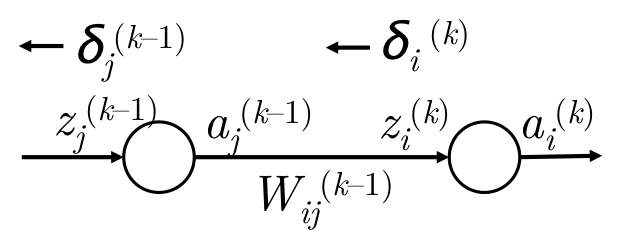
\includegraphics[width=\linewidth]{ErrorSignal2}
  \caption{Propagating error from $\delta^{(k)}$ to $\delta^{(k-1)}$}
  \label{fig:ErrorSignal2}
\end{marginfigure}

\begin{enumerate}
\item We have error $\delta^{(k)}_i$ propagating backwards from $z^{(k)}_i$, i.e. neuron $i$ at layer $k$. See Figure~\ref{fig:ErrorSignal2}.
\item We propagate this error backwards to $a^{(k-1)}_j$ by multiplying $\delta^{(k)}_i$ by the path weight $W^{(k-1)}_{ij}$.
\item Thus, the error received at $a^{(k-1)}_j$ is $\delta^{(k)}_i W^{(k-1)}_{ij}$.
\item However, $a^{(k-1)}_j$ may have been forwarded to multiple nodes in the next layer as shown in Figure~\ref{fig:ErrorSignal3}. It should receive responsibility for errors propagating backward from node $m$ in layer $k$ too, using the exact same mechanism.
\item Thus, error received at $a^{(k-1)}_j$ is $\delta^{(k)}_i W^{(k-1)}_{ij} + \delta^{(k)}_m W^{(k-1)}_{mj}$.
\item In fact, we can generalize this to be $\sum_i \delta^{(k)}_i W^{(k-1)}_{ij}$.
\item Now that we have the correct error at $a^{(k-1)}_j$, we move it across neuron $j$ at layer $k-1$ by multiplying with with the local gradient $f'(z_j^{(k-1)})$.
\item Thus, the error that reaches $z_j^{(k-1)}$, called $\delta_j^{(k-1)}$ is \\$f'(z_j^{(k-1)}) \sum_i \delta^{(k)}_i W^{(k-1)}_{ij}$
\end{enumerate}

\begin{marginfigure}%
  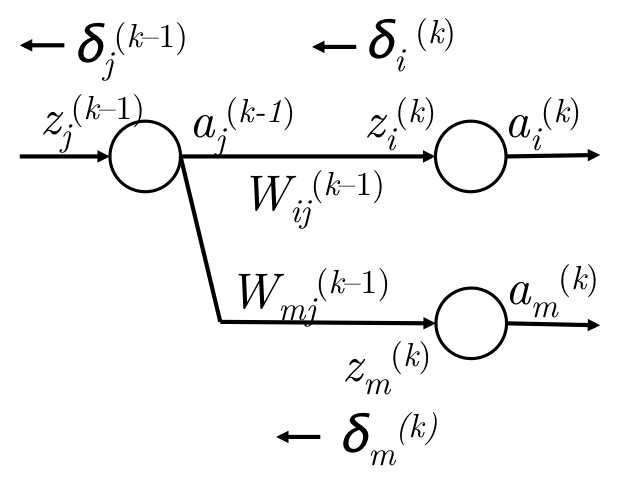
\includegraphics[width=\linewidth]{ErrorSignal3}
  \caption{Propagating error from $\delta^{(k)}$ to $\delta^{(k-1)}$}
  \label{fig:ErrorSignal3}
\end{marginfigure}

\subsection{Training with Backpropagation -- Vectorized}\label{sec:backprop2}

So far, we discussed how to calculate gradients for a given parameter in the model. Here we will generalize the approach above so that we update weight matrices and bias vectors all at once. Note that these are simply extensions of the above model that will help build intuition for the way error propagation can be done at a matrix-vector level.

For a given parameter $W_{ij}^{(k)}$, we identified that the error gradient is simply $\delta_{i}^{(k+1)}\cdot a_j^{(k)}$. As a reminder, $W^{(k)}$ is the matrix that maps $a^{(k)}$ to $z^{(k+1)}$. We can thus establish that the error gradient for the entire matrix $W^{(k)}$ is: 
$$ \nabla_{W^{(k)}} = \begin{bmatrix} \delta_{1}^{(k+1)} a_1^{(k)} & \delta_{1}^{(k+1)} a_2^{(k)} & \cdots \\ \delta_{2}^{(k+1)} a_1^{(k)} & \delta_{2}^{(k+1)} a_2^{(k)} & \cdots \\ \vdots & \vdots & \ddots \end{bmatrix} = \delta^{(k+1)} a^{(k)T}$$

\marginnote{\textbf{Error propagates} from layer $(k+1)$ to $(k)$ in the following manner:
$$\delta^{(k)} = f'(z^{(k)}) \circ (W^{(k)T} \delta^{(k+1)})$$
Of course, this assumes that in the forward propagation the signal $z^{(k)}$ first goes through activation neurons $f$ to generate activations $a^{(k)}$ and are then linearly combined to yield $z^{(k+1)}$ via transfer matrix $W^{(k)}$.}

Thus, we can write an entire matrix gradient using the outer product of the error vector propagating into the matrix and the activations forwarded by the matrix.

Now, we will see how we can calculate the error vector $\delta^{(k)}$. We established earlier using Figure~\ref{fig:ErrorSignal3} that $\delta^{(k)}_j =f'(z_j^{(k)}) \sum_i \delta^{(k+1)}_i W^{(k)}_{ij}$. This can easily generalize to matrices such that:
$$\delta^{(k)} = f'(z^{(k)}) \circ (W^{(k)T} \delta^{(k+1)}) $$
In the above formulation, the $\circ$ operator corresponds to an element wise product between elements of vectors ($\circ : \mathbb{R}^N \times \mathbb{R}^N \rightarrow \mathbb{R}^N$).
$$ $$
\textbf{Computational efficiency:} Having explored element-wise updates as well as vector-wise updates, we must realize that the vectorized implementations run substantially faster in scientific computing environments such as MATLAB or Python (using NumPy/SciPy packages). Thus, we should use vectorized implementation in practice. Furthermore, we should also reduce redundant calculations in backpropagation - for instance, notice that $\delta^{(k)}$ depends directly on $\delta^{(k+1)}$. Thus, we should ensure that when we update $W^{(k)}$ using $\delta^{(k+1)}$, we save $\delta^{(k+1)}$ to later derive $\delta^{(k)}$ -- and we then repeat this for $(k-1)\hdots(1)$. Such a recursive procedure is what makes backpropagation a computationally affordable procedure.

\section{Neural Networks: Tips and Tricks}\label{sec:nnetstips}

Having discussed the mathematical foundations of neural networks, we will now dive into some tips and tricks commonly employed when using neural networks in practice.

\subsection{Gradient Check}
In the last section, we discussed in detail how to calculate error gradients/updates for parameters in a neural network model via calculus-based (analytic) methods. Here we now introduce a technique of \textit{numerically} approximating these gradients -- though too computationally inefficient to be used directly for training the networks, this method will allow us to very precisely estimate the derivative with respect to any parameter; it can thus serve as a useful sanity check on the correctness of our analytic derivatives. Given a model with parameter vector $\theta$ and loss function $J$, the numerical gradient around $\theta_i$ is simply given by \textbf{centered difference formula}:

$$ f'(\theta) \approx \frac{J(\theta^{(i+)}) - J(\theta^{(i-)})}{2 \epsilon}$$
where $\epsilon$ is a small number (usually around $1e^{-5}$). The term $J(\theta^{(i+)})$ is simply the error calculated on a forward pass for a given input when we perturb the parameter $\theta$'s $i^{th}$ element by $+\epsilon$. Similarly, the term $J(\theta^{(i-)})$ is the error calculated on a forward pass for the same input when we perturb the parameter $\theta$'s $i^{th}$ element by $-\epsilon$. Thus, using two forward passes, we can approximate the gradient with respect to any given parameter element in the model. We note that this definition of the numerical gradient follows very naturally from the definition of the derivative, where, in the scalar case,

$$f'(x) \approx \dfrac{f(x + \epsilon) - f(x)}{\epsilon}$$

\marginnote{\textbf{Gradient checks} are a great way to compare analytical and numerical gradients. Analytical gradients should be close and numerical gradients can be calculated using: $$ f'(\theta) \approx \frac{J(\theta^{(i+)}) - J(\theta^{(i-)})}{2 \epsilon}$$ $J(\theta^{(i+)})$ and $J(\theta^{(i-)})$ can be evaluated using two forward passes. An implementation of this can be seen in Snippet~\ref{snip:gradcheck}.}

Of course, there is a slight difference -- the definition above only perturbs $x$ in the positive direction to compute the gradient. While it would have been perfectly acceptable to define the numerical gradient in this way, in practice it is often more precise and stable to use the {centered difference formula}, where we perturb a parameter in both directions. The intuition is that to get a better approximation of the derivative/slope around a point, we need to examine the function $f$'s behavior both to the left and right of that point. It can also be shown using Taylor's theorem that the centered difference formula has an error proportional to $\epsilon^2$, which is quite small, whereas the derivative definition is more error-prone.

Now, a natural question you might ask is, if this method is so precise, why do we not use it to compute all of our network gradients instead of applying back-propagation? The simple answer, as hinted earlier, is inefficiency -- recall that every time we want to compute the gradient with respect to an element, we need to make two forward passes through the network, which will be computationally expensive. Furthermore, many large-scale neural networks can contain millions of parameters, and computing two passes per parameter is clearly not optimal. And, since in optimization techniques such as SGD, we must compute the gradients once per iteration for several thousands of iterations, it is obvious that this method quickly grows intractable. This inefficiency is why we only use gradient check to verify the correctness of our analytic gradients, which are much quicker to compute. A standard implementation of gradient check is shown below:


% f course, considering how many operations are required for even a forward pass, this is an extremely expensive procedure of evaluating gradients -- as stated eariler, however, is a great way of verifying implementations of the backpropagation however.
\begin{theorem}
\begin{verbatim}

def eval_numerical_gradient(f, x):
  """ 
  a naive implementation of numerical gradient of f at x 
  - f should be a function that takes a single argument
  - x is the point (numpy array) to evaluate the gradient 
  at
  """ 

  fx = f(x) # evaluate function value at original point
  grad = np.zeros(x.shape)
  h = 0.00001

  # iterate over all indexes in x
  it = np.nditer(x, flags=['multi_index'], 
  	                op_flags=['readwrite'])
  while not it.finished:

    # evaluate function at x+h
    ix = it.multi_index
    old_value = x[ix]
    x[ix] = old_value + h # increment by h
    fxh_left = f(x) # evaluate f(x + h)
    x[ix] = old_value - h # decrement by h
    fxh_right = f(x) # evaluate f(x - h)
    x[ix] = old_value # restore to previous value (very 
    			      important!)

    # compute the partial derivative
    grad[ix] = (fxh_left - fxh_right) / (2*h) # the slope
    it.iternext() # step to next dimension
  return grad  
\end{verbatim}
\label{snip:gradcheck}
\end{theorem}
\subsection{Regularization}

As with many machine learning models, neural networks are highly prone to overfitting, where a model is able to obtain near perfect performance on the training dataset, but loses the ability to generalize to unseen data. A common technique used to address overfitting (an issue also known as the ``high-variance problem'') is the incorporation of an $L_2$ regularization penalty. The idea is that we will simply append an extra term to our loss function $J$, so that the overall cost is now calculated as:

$$J_R = J + \lambda \sum_{i = 1}^{L} \norm{W^{(i)}}_F$$

\marginnote{The \textbf{Frobenius Norm} of a matrix $U$ is defined as follows:
$$||U||_F = \sqrt{ \sum_{i}\sum_{j}U_{ij}^2 }$$
}

In the above formulation, $\norm{W^{(i)}}_F$ is the Frobenius norm of the matrix $W^{(i)}$ (the $i$-th weight matrix in the network) and $\lambda$ is the hyper-parameter controlling how much weight the regularization term has relative to the original cost function. Since we are trying to minimize $J_R$, what regularization is essentially doing is penalizing weights for being too large while optimizing over the original cost function. Due to the quadratic nature of the Frobenius norm (which computes the sum of the squared elements of a matrix), $L_2$-regularization effectively reduces the flexibility of the model and thereby reduces the overfitting phenomenon. Imposing such a constraint can also be interpreted as the prior Bayesian belief that the optimal weights are close to zero -- how close depends on the value of $\lambda$. Choosing the right value of $\lambda$ is critical, and must be chosen via hyperparameter-tuning. Too high a value of $\lambda$ causes most of the weights to be set too close to $0$, and the model does not learn anything meaningful from the training data, often obtaining poor accuracy on training, validation, and testing sets. Too low a value, and we fall into the domain of overfitting once again. It must be noted that the bias terms are not regularized and do not contribute to the cost term above -- try thinking about why this is the case!

There are indeed other types of regularization that are sometimes used, such as $L_1$ regularization, which sums over the absolute values (rather than squares) of parameter elements -- however, this is less commonly applied in practice since it leads to sparsity of parameter weights. In the next section, we discuss \textit{dropout}, which effectively acts as another form of regularization by randomly dropping (i.e. setting to zero) neurons in the forward pass.

\subsection{Dropout}

Dropout is a powerful technique for regularization, first introduced by Srivastava et al. in \textit{Dropout: A Simple Way to Prevent Neural Networks from Overfitting}.  The idea is simple yet effective -- during training, we will randomly ``drop'' with some probability $(1-p)$ a subset of neurons during each forward/backward pass (or equivalently, we will keep alive each neuron with a probability $p$). Then, during testing, we will use the full network to compute our predictions. The result is that the network typically learns more meaningful information from the data, is less likely to overfit, and usually obtains higher performance overall on the task at hand. One intuitive reason why this technique should be so effective is that what dropout is doing is essentially doing is training exponentially many smaller networks at once and averaging over their predictions. 


\marginnote{
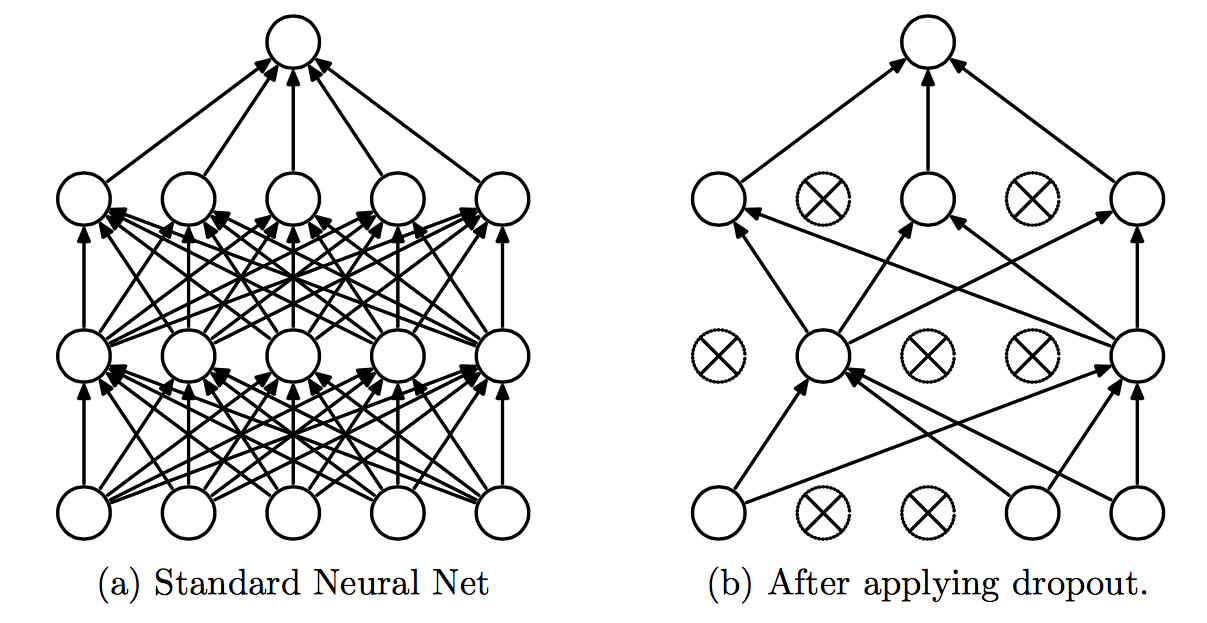
\includegraphics[width=6cm]{dropout.png}
{Dropout applied to an artificial neural network. Image credits to Srivastava et al.}
}


In practice, the way we introduce dropout is that we take the output $h$ of each layer of neurons, and keep each neuron with probability $p$, and else set it to $0$. Then, during back-propagation, we only pass gradients through neurons that were kept alive during the forward pass. Finally, during testing, we compute the forward pass using \textit{all} of the neurons in the network. However, a key subtlety is that in order for dropout to work effectively, the expected output of a neuron during testing should be approximately the same as it was during training -- else the magnitude of the outputs could be radically different, and the behavior of the network is no longer well-defined. Thus, we must typically divide the outputs of each neuron during testing by a certain value -- it is left as an exercise to the reader to determine what this value should be in order for the expected outputs during training and testing to be equivalent.

\subsection{Neuron Units}

So far we have discussed neural networks that contain sigmoidal neurons to introduce nonlinearities; however in many applications better networks can be designed using other activation functions. Some common choices are listed here with their function and gradient definitions and these can be substituted with the sigmoidal functions discussed above.
$$ $$
\textbf{Sigmoid:} This is the default choice we have discussed; the activation function $\sigma$ is given by:
\begin{marginfigure}%
  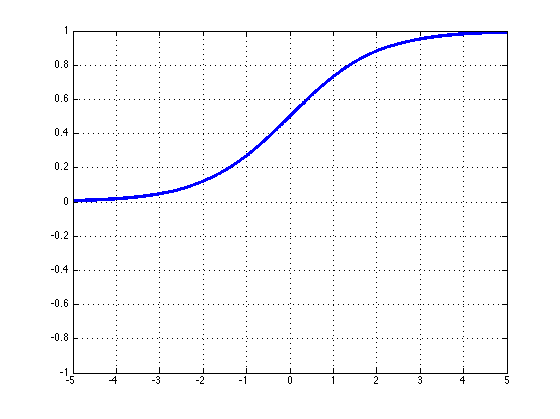
\includegraphics[width=\linewidth]{graph_sigmoid}
  \caption{The response of a sigmoid nonlinearity}
  \label{fig:graph_sigmoid}
\end{marginfigure}
\begin{align*}
  \sigma(z) &= \frac{1}{1 + \operatorname{exp}(-z)}\\
  \text{where}~\sigma(z) &\in (0, 1)
\end{align*}
The gradient of $ \sigma(z) $ is:
$$ \sigma'(z) = \frac{- \operatorname{exp}(-z)}{1 +  \operatorname{exp}(-z)} = \sigma(z) (1 - \sigma(z))$$
\textbf{Tanh:} The tanh function is an alternative to the sigmoid function that is often found to converge faster in practice. The primary difference between tanh and sigmoid is that tanh output ranges from $-1$ to $1$ while the sigmoid ranges from $0$ to $1$.
\begin{marginfigure}%
  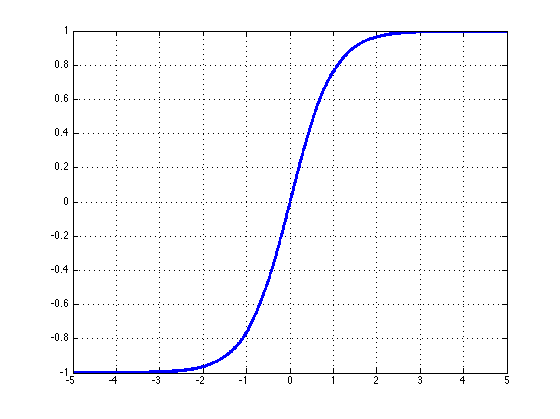
\includegraphics[width=\linewidth]{graph_tanh}
  \caption{The response of a tanh nonlinearity}
  \label{fig:graph_tanh}
\end{marginfigure}
\begin{align*}
  \operatorname{tanh}(z) &=  \frac{\operatorname{exp}(z) - \operatorname{exp}(-z)}{\operatorname{exp}(z) + \operatorname{exp}(-z)} = 2\sigma(2z) - 1\\
  \text{where}~\operatorname{tanh}(z) &\in (-1, 1)
\end{align*}
The gradient of $ \operatorname{tanh}(z) $ is:
$$ \operatorname{tanh}'(z) = 1 - \bigg(\frac{\operatorname{exp}(z) - \operatorname{exp}(-z)}{\operatorname{exp}(z) + \operatorname{exp}(-z)}\bigg)^2 = 1 - \operatorname{tanh}^2(z)$$
\textbf{Hard tanh:}
The hard tanh function is sometimes preferred over the tanh function since it is computationally cheaper. It does however saturate for magnitudes of $z$ greater than $1$. The activation of the hard tanh is:
\begin{marginfigure}%
  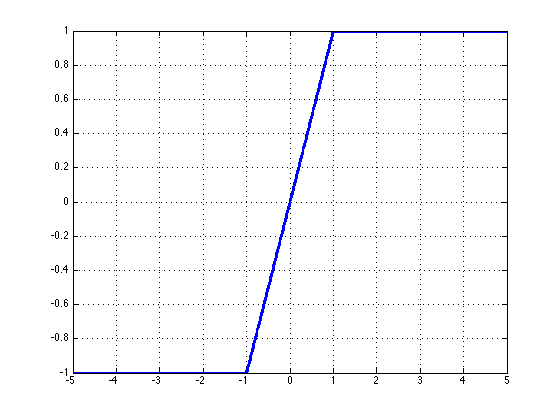
\includegraphics[width=\linewidth]{graph_hardtanh}
  \caption{The response of a hard tanh nonlinearity}
  \label{fig:graph_hardtanh}
\end{marginfigure}
\begin{displaymath}
    \operatorname{hardtanh}(z) = \left\{
     \begin{array}{cl}
       -1 & : z < -1\\
       z & : -1 \leq z \leq 1\\
       1 & : z > 1
     \end{array}
   \right.
\end{displaymath} 
The derivative can also be expressed in a piecewise functional form:
\begin{displaymath}
    \operatorname{hardtanh}'(z) = \left\{
     \begin{array}{cl}
       1 & : -1 \leq z \leq 1\\
       0 & : \text{otherwise}
     \end{array}
   \right.
\end{displaymath} 
\textbf{Soft sign:}
The soft sign function is another nonlinearity which can be considered an alternative to tanh since it too does not saturate as easily as hard clipped functions:
\begin{marginfigure}%
  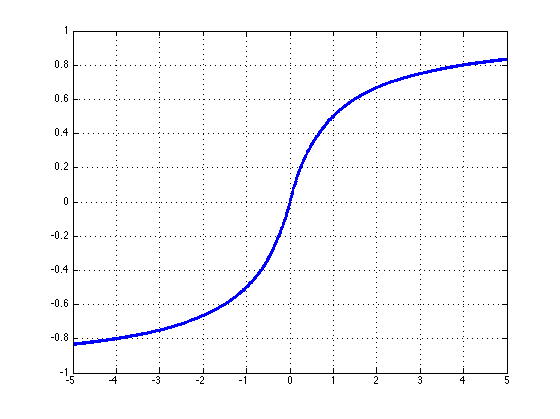
\includegraphics[width=\linewidth]{graph_softsign}
  \caption{The response of a soft sign nonlinearity}
  \label{fig:graph_softsign}
\end{marginfigure}
$$\operatorname{softsign}(z) = \frac{z}{1 + |z|}$$
The derivative is the expressed as:
$$\operatorname{softsign}'(z) = \frac{\operatorname{sgn}(z)}{(1 + z)^2}$$
$$\text{where}~\operatorname{sgn} \text{ is the signum function which returns }\pm1\text{ depending on the sign of }z$$
$$ $$
\textbf{ReLU:} The ReLU (Rectified Linear Unit) function is a popular choice of activation since it does not saturate even for larger values of $z$ and has found much success in computer vision applications:
\begin{marginfigure}%
  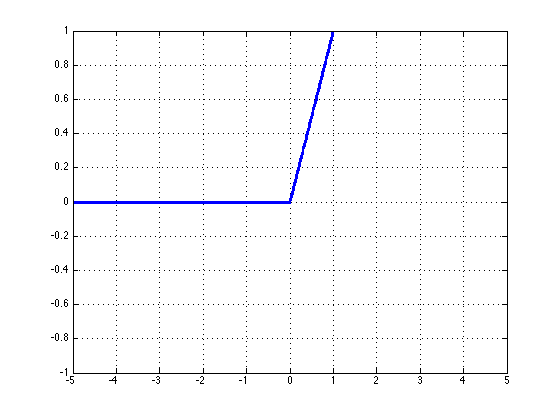
\includegraphics[width=\linewidth]{graph_relu}
  \caption{The response of a ReLU nonlinearity}
  \label{fig:graph_relu}
\end{marginfigure}
$$\operatorname{rect}(z) = \operatorname{max}(z, 0)$$
The derivative is then the piecewise function:
\begin{displaymath}
    \operatorname{rect}'(z) = \left\{
     \begin{array}{cl}
       1 & : z > 0\\
       0 & : \text{otherwise}
     \end{array}
   \right.
\end{displaymath} 
\textbf{Leaky ReLU:} Traditional ReLU units by design do not propagate any error for non-positive $z$ -- the leaky ReLU modifies this such that a small error is allowed to propagate backwards even when $z$ is negative:

\begin{marginfigure}%
  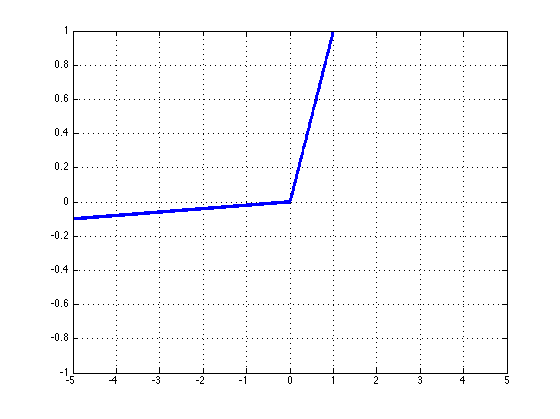
\includegraphics[width=\linewidth]{graph_leaky}
  \caption{The response of a leaky ReLU nonlinearity}
  \label{fig:graph_leaky}
\end{marginfigure}

$$\operatorname{leaky}(z) = \operatorname{max}(z, k\cdot z)$$
$$\text{where } 0<k<1$$
This way, the derivative is representable as:
\begin{displaymath}
    \operatorname{leaky}'(z) = \left\{
     \begin{array}{cl}
       1 & : z > 0\\
       k & : \text{otherwise}
     \end{array}
   \right.
\end{displaymath} 

\subsection{Data Preprocessing}
As is the case with machine learning models generally, a key step to ensuring that your model obtains reasonable performance on the task at hand is to perform basic preprocessing on your data. Some common techniques are outlined below.\\
\vspace{6mm}

\noindent\textbf{Mean Subtraction}\\

\noindent{}Given a set of input data $X$, it is customary to zero-center the data by subtracting the mean feature vector of $X$ from $X$. An important point is that in practice, the mean is calculated only across the training set, and this mean is subtracted from the training, validation, and testing sets.\\
\vspace{6mm}

\noindent\textbf{Normalization}\\

\noindent{}Another frequently used technique (though perhaps less so than mean subtraction) is to scale every input feature dimension to have similar ranges of magnitudes. This is useful since input features are often measured in different ``units'', but we often want to initially consider all features as equally important. The way we accomplish this is by simply dividing the features by their respective standard deviation calculated across the training set.\\
\vspace{6mm}

\noindent\textbf{Whitening}\\

\noindent{}Not as commonly used as mean-subtraction + normalization, whitening essentially converts the data to a have an identity covariance matrix -- that is, features become uncorrelated and have a variance of $1$.  This is done by first mean-subtracting the data, as usual, to get $X'$. We can then take the Singular Value Decomposition (SVD) of $X'$ to get matrices $U, S, V$. We then compute $UX'$ to project  $X'$ into the basis defined by the columns of $U$. We finally divide each dimension of the result by the corresponding singular value in $S$ to scale our data appropriately (if a singular value is zero, we can just divide by a small number instead).


\subsection{Parameter Initialization}

A key step towards achieving superlative performance with a neural network is initializing the parameters in a reasonable way.  A good starting strategy is to initialize the weights to small random numbers normally distributed around $0$ -- and in practice, this often words acceptably well.
However, in \textsc{Understanding the difficulty of training deep feedforward neural networks (2010), Xavier et al} study the effect of different weight and bias initialization schemes on training dynamics. The empirical findings suggest that for sigmoid and tanh activation units, faster convergence and lower error rates are achieved when the weights of a matrix $W \in \mathbb{R}^{n^{(l+1)}\times n^{(l)}}$ are initialized randomly with a uniform distribution as follows:
$$W \sim U\bigg[-\sqrt{\frac{6}{n^{(l)} + n^{(l+1)}}}, \sqrt{\frac{6}{n^{(l)} + n^{(l+1)}}}\bigg]$$
Where $n^{(l)}$ is the number of input units to $W$ (fan-in) and  $n^{(l+1)}$ is the number of output units from $W$ (fan-out).
In this parameter initialization scheme, bias units are initialized to $0$. This approach attempts to maintain activation variances as well as backpropagated gradient variances across layers. Without such initialization, the gradient variances (which are a proxy for information) generally decrease with backpropagation across layers.
\subsection{Learning Strategies}
The rate/magnitude of model parameter updates during training can be controlled using the learning rate. In the following naive Gradient Descent formulation, $\alpha$ is the learning rate:
$$ \theta^{\text{new}} = \theta^{\text{old}} - \alpha \nabla_{\theta}J_t(\theta)$$
You might think that for fast convergence rates, we should set $\alpha$ to larger values -- however faster convergence is not guaranteed with larger convergence rates. In fact, with very large learning rates, we might experience that the loss function actually diverges because the parameters update causes the model to overshoot the convex minima as shown in Figure~\ref{fig:ErrorSurf}. In non-convex models (most of those we work with), the outcome of a large learning rate is unpredictable, but the chances of diverging loss functions are very high.

\begin{marginfigure}%
  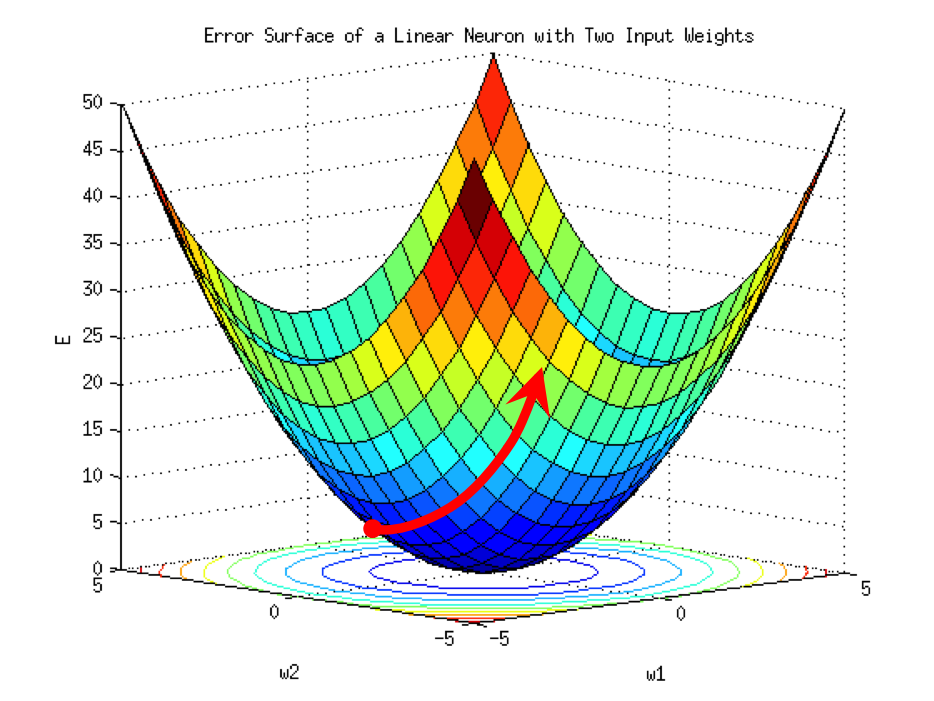
\includegraphics[width=\linewidth]{Error_Surf}
  \caption{Here we see that updating parameter $w_2$ with a large learning rate can lead to divergence of the error.}
  \label{fig:ErrorSurf}
\end{marginfigure}

The simple solution to avoiding a diverging loss is to use a very small learning rate so that we carefully scan the parameter space -- of course, if we use too small a learning rate, we might not converge in a reasonable amount of time, or might get caught in local minima.  Thus, as with any other hyperparameter, the learning rate must be tuned effectively.

% Furthermore, we can keep this learning rate fixed for all parameters in the model instead of having a more complex scheme in which each parameter has its own learning rate.

Since training is the most expensive phase in a deep learning system, some research has attempted to improve this naive approach to setting learning learning rates. For instance, \textsc{Ronan Collobert} scales the learning rate of a weight $W_{ij}$  (where $W \in \mathbb{R}^{n^{(l+1)}\times n^{(l)}}$) by the inverse square root of the fan-in of the neuron ($n^{(l)}$). 

There are several other techniques that have proven to be effective as well -- one such method is \textbf{annealing}, where, after several iterations, the learning rate is reduced in some way -- this method ensures that we start off with a high learning rate and approach a minimum quickly; as we get closer to the minimum, we start lowering our learning rate so that we can find the optimum under a more fine-grained scope. A common way to perform annealing is to reduce the learning rate $\alpha$ by a factor $x$ after every $n$ iterations of learning. Exponential decay is also common, where, the learning rate $\alpha$ at iteration $t$ is given by $\alpha(t) = \alpha_0e^{-kt}$, where $\alpha_0$ is the initial learning rate, and $k$ is a hyperparameter. Another approach is to allow the learning rate to decrease over time such that:
$$ \alpha(t) = \frac{\alpha_0\tau}{\max(t, \tau)}$$
In the above scheme, $\alpha_0$ is a tunable parameter and represents the starting learning rate. $\tau$ is also a tunable parameter and represents the time at which the learning rate should start reducing. In practice, this method has been found to work quite well. In the next section we discuss another method for adaptive gradient descent which does not require hand-set learning rates.


\subsection{Momentum Updates}

Momentum methods, a variant of gradient descent inspired by the study of dynamics and motion in physics, attempt to use the ``velocity'' of updates as a more effective update scheme. Pseudocode for momentum updates is shown below:

\begin{theorem}
\begin{verbatim}

# Computes a standard momentum update
# on parameters x
v = mu*v - alpha*grad_x
x += v
\end{verbatim}
\label{snip:momentup}
\end{theorem}


\subsection{Adaptive Optimization Methods}

AdaGrad is an implementation of standard stochastic gradient descent (SGD) with one key difference: the learning rate can vary for each parameter. The learning rate for each parameter depends on the history of gradient updates of that parameter in a way such that parameters with a scarce history of updates are updated faster using a larger learning rate. In other words, parameters that have not been updated much in the past are likelier to have higher learning rates now. Formally:

$$\theta_{t,i} = \theta_{t-1,i}  - \frac{\alpha}{\sqrt{\sum_{\tau=1}^{t} g_{\tau , i}^2}} g_{t,i} \text{ where } g_{t,i} = \frac{\partial}{\partial \theta_i^t}J_t(\theta) $$

In this technique, we see that if the RMS of the history of gradients is extremely low, the learning rate is very high. A simple implementation of this technique is:
\begin{theorem}
\begin{verbatim}

# Assume the gradient dx and parameter vector x
cache += dx**2
x += - learning_rate * dx / np.sqrt(cache + 1e-8)
\end{verbatim}
\label{snip:adagrad}
\end{theorem}
Other common adaptive methods are RMSProp and Adam, whose update rules are shown below (courtesy of Andrej Karpathy):

\begin{theorem}
\begin{verbatim}

# Update rule for RMS prop
cache = decay_rate * cache + (1 - decay_rate) * dx**2
x += - learning_rate * dx / (np.sqrt(cache) + eps)
\end{verbatim}
\label{snip:rmsprop}
\end{theorem}

\begin{theorem}
\begin{verbatim}

# Update rule for Adam
m = beta1*m + (1-beta1)*dx
v = beta2*v + (1-beta2)*(dx**2)
x += - learning_rate * m / (np.sqrt(v) + eps)
\end{verbatim}
\label{snip:adam}
\end{theorem}
RMSProp is a variant of AdaGrad that utilizes a moving average of squared gradients -- in particular, unlike AdaGrad, its updates do not become monotonically smaller. The Adam update rule is in turn a variant of RMSProp, but with the addition of momentum-like updates. We refer the reader to the respective sources of these methods for more detailed analyses of their behavior.






\end{document}
